The driving principle behind our strategic plan can be summarized as
``Benchmark, then improve.'' We are analyzing a real-world system
(that of fans traveling to and form the stadium), and we are building
our own software system to simulate it. Our project will therefore
first focus on computing `sensible' emissions values for an average
game, and will then develop a full software model to quantify the
impact of different policies that could be put in place. In
engineering terms, we are first calculating the equilibrium or
``trim'' condition and then we will focus on disturbances away from
it.

\subsection{System Proposed Approach}
The approach to both problems will of necessity be similar, and our
aim is to design our solution to the first problem with a great deal
of flexibility so that it may be readily adapted for use in the second
phase of the project. Our phase 1 model will have five main components
that correspond to the four steps of the UTMS plus a GHG
calculator. The blocks described below correspond to the block diagram
shown in figure \ref{mainsystem1}.

\begin{figure}[htp]
  \centering
  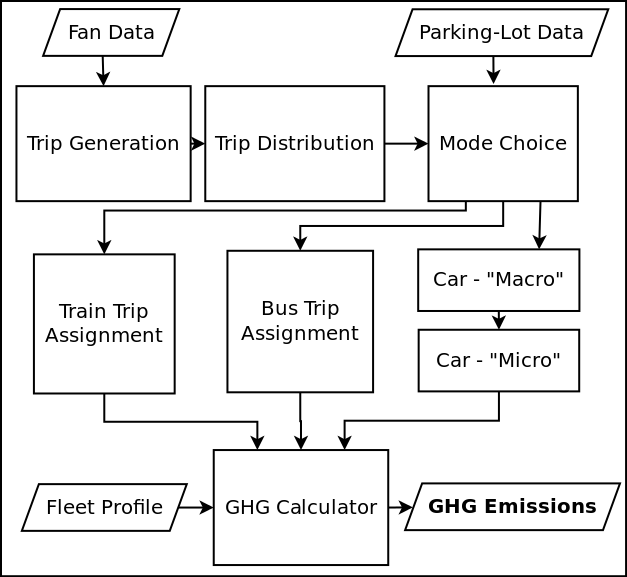
\includegraphics[height=8cm]{graphics/fullsystem1.png}
  \caption{System block diagram of our phase 1 model}
  \label{mainsystem1}
\end{figure}

\begin{description}[style=nextline]
    \item[Trip Generation] We will need to gather data on the
  geographic distribution of the fans that attend the games. We hope
  to obtain a good amount of data from the Eagles to aid in this
  section. Absent that data, we will have to resort to theoretical
  models commonly used in the industry, such as the Gravity Model. We
  will also be gathering data on timing of the trips, either through
  direct observation, or ideally from already existing records.
    \item[Trip Distribution] This step in the modeling is
  straightforward, since we know that fans are traveling to and from
  the stadium (or a nearby parking lot).
    \item[Mode Choice] This phase involves matching each trip in the
  database to a mode of travel (i.e. Car vs. SEPTA vs. Bus). We plan
  on using parking-lot data to estimate car use, and, if possible, get
  station-level information directly from SEPTA. A variety of
  theoretical models exist to help validate the gathered data.
    \item[Trip Assignment] Is the selection of the specific lines,
  streets, highways, and stations that each trip will follow. At this
  stage, we will break the model into subsystems for each of the
  possible means of transportation.
    \begin{description}[style=nextline]
        \item[Trains] A great deal of information is available on the
      website regarding lines and schedules that we have used to build
      a software representation of the network. With some
      well-established linear optimization algorithms, we will be able
      to model the exact path taken for every trip assigned to SEPTA
      trains. A preliminary step is to populate the station model, as
      shown in figure \ref{septa-db}. Then, we will use established
      algorithms to run the model based on this database, as shown in
      figure \ref{septa}
        \item[Buses] Schedules and stops are also available at
      www.septa.org. We will merge this database with the
      information available on Google Maps to obtain location data.
      There are also well-established algorithms we can use to model
      the paths of every trip.
        \item[Cars] Our car model will be split in two: \label{cars}
      \begin{itemize}
          \item At a "micro" level, we will model the road network in
        and around the stadium parking lot based on existing databases
        complemented with hand-input data that we extract from maps
        and planning documents. This portion will be used to model the
        exiting cars, since we believe the congestion at the end of a
        game results in substantial GHG emissions.
          \item At a "macro" level, we will use the same TAZs as in
        the trip generation phase, and calculate a sample path to the
        stadium based on highways and main roads.  We will have to
        encode the network of such roads and use our own algorithms.
        Alternatively, depending on the resulting number of TAZs, and
        subject to special authorization, we could use the Google Maps
        API to programmatically retrieve routing information.
      \end{itemize}
    \end{description}
      \item[GHG Calculator] This subsystem will be a memoryless
    function mapping a trip to an estimated emissions value. Our
    preliminary assumption is that trips taken on public transit
    contribute no additional GHG, since we are taking the bus and
    train schedules as given. For cars, there are a multitude of
    published methods for estimating emissions. We will have to
    estimate a fleet profile (average age and size) to use one of
    these models. We expect that it will be a function of total
    highway distance/time, local street distance/time, and idling
    time. When properly built, the output from this subsystem will be
    our first main deliverable.
\end{description}

\begin{figure}[htp]
  \centering
  \begin{subfigure}{.504\textwidth}
    \centering
    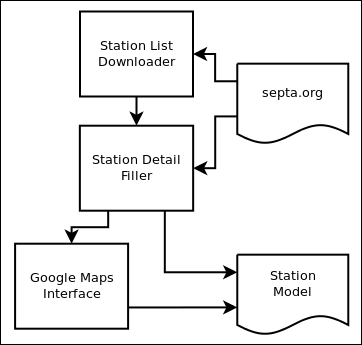
\includegraphics[width=\textwidth]{graphics/septa-db.png}
    \caption{Populating the station database}
    \label{septa-db}
  \end{subfigure}
    \begin{subfigure}{.394\textwidth}
    \centering
    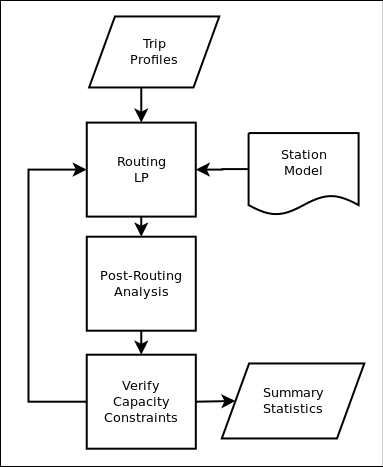
\includegraphics[width=\textwidth]{graphics/septa.png}
    \caption{Operation of the train subsystem}
    \label{septa}
  \end{subfigure}
  \caption{Components of the SEPTA Train Model}
% septa.png 383 w x 467 h
% septa-db.png 362 w x 345 h
% w1 * 467 / 383 = w2 * 345 / 362
% w2 = w1 * (467 * 362) / (383 * 345) = w1 * 1.2794
% w1 + w2 = .9\textwidth
% w1 = .9\textwidth / ( 2.27924)
%    = .394\textwidth
% w2 = .504\textwidth
\end{figure}

For the second phase of the project, as mentioned above, we will seek
to leverage as much of the modeling work from phase one as
possible. The goal for this phase will be to focus on converting the
existing model into a usable simulator. A key objective will be
incorporating a variety of inter-system feedback mechanisms that will
allow for a more accurate model.  The degree of detail in these
feedbacks mechanism will be constrained by the computational
complexity of including them (see Table \ref{specs} for computational
requirements) and by the design constraints of our subsystems (see
Section \ref{requirements}) Since there may be limited opportunities
to validate our model (until the next season begins), a key
performance metric will be the consistency of results, which in
technical terms, means that the system should reject small
disturbances in the inputs.  Conceptually, changing the base fare for
SEPTA or increasing the cost of parking by small amounts should not
result in wildly different behavior. This sensitivity will be a key
measure we will use in determining the right level of complexity to
build into the model.

Some examples of feedback mechanisms we are considering at this stage
are:

\begin{description}[style=nextline]
    \item[Congestion] If a fan spends 45 minutes stuck in the parking
  lot unable to move, we expect that fan to be more likely to take the
  train for the next game. A more detailed discussion of the fan model
  lies below.
    \item[Scheduling] If SEPTA notices trains traveling fuller on game
  days, they may choose to alter schedules in the future.
    \item[Uncertainty Effects] As fans try different modes of
  transportation, they may refine their predictions of travel times
  and convenience.
    \item[Fleet Composition] We suspect the fans that are most likely
  to start using public transit may have cars with above-average fuel
  efficiency, whereas the fans that take their trucks to tail-gate
  parties will likely continue to use their less-efficient cars.
  These effects would alter the fleet profile and hence average
  emissions calculations.
\end{description}

Regardless of what feedback loops we ultimately incorporate, we will
have to build a model of the fans' utilities, to capture the effects
of the various incentive schemes on trip generation profiles. At this
stage we expect we will be using an agent-based technique for this
subsystem, which will have as inputs the TAZs and some demographic
data. Cooperation from the Eagles will be important in fine-tuning
this part of the model.

The expanded model can be seen in the block diagram in figure
\ref{mainsystem2}. We have included the incentive structure as an
input in the diagram. We expect to make a GUI for this input to the
model, which will have a variety of options. For now, we have left
these unspecified as we will have to discuss with the Eagles what
their interests are. The other block added is the preference model,
which will be an agent- or automata-based model about fan preferences,
i.e. how they value travel time, convenience, comfort, and other
parameters that differ between the different modes of transportation.

\begin{figure}[htp]
  \centering
  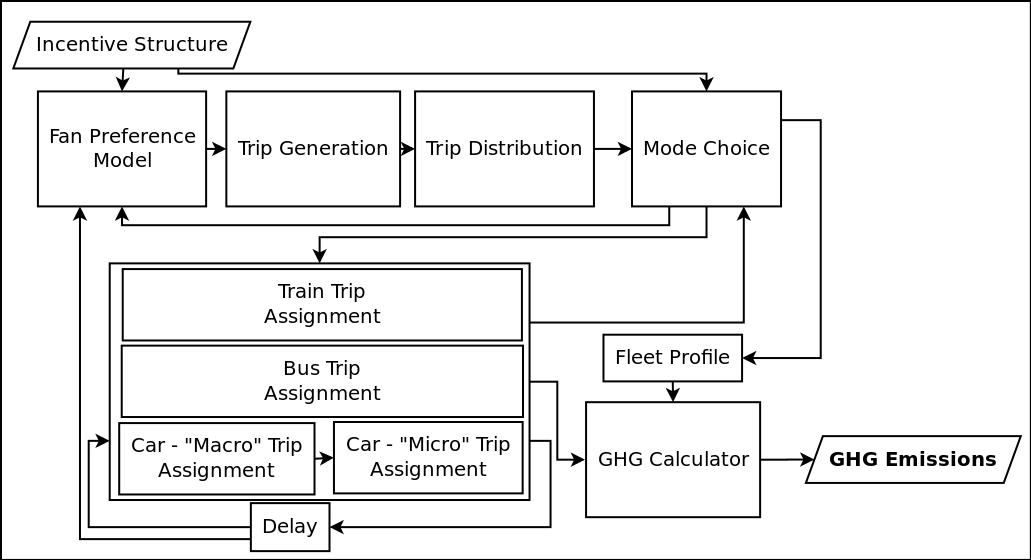
\includegraphics[height=8cm]{graphics/fullsystem2.png}
  \caption{Full system incorporating feedback}
  \label{mainsystem2}
\end{figure}

